\documentclass{mcmthesis}

\usepackage{subcaption}
\usepackage{graphicx}

\mcmsetup{CTeX = false,    % 使用 CTeX 套装时,设置为 true
          tcn = {240718}, problem = \textcolor{red}{C},
          sheet = true, titleinsheet = true, keywordsinsheet = true,
          titlepage = false, abstract = false}
		
\usepackage{newtxtext}	%Palatino的字体宏包
\usepackage[style=apa,backend=biber]{biblatex}	%参考文献排版引擎
\addbibresource{test1_reference.bib}	%添加参考文献数据库

\usepackage{tocloft}	%修改目录 ,,,,
\setlength{\cftbeforesecskip}{6pt}	%设置章节标题在目录里的垂直距离
\renewcommand{\contentsname}{\hspace*{\fill}\Large\bfseries Contents \hspace*{\fill}}	%修改目录标题显示方式{\控制标题文本}{\水平居中}\大号字体\粗体

\title{\bf Quantifying momentum, grasping victory in tennis}
\date{\today}

\begin{document}

\begin{abstract}

Physics defines where momentum as “the strength or force gained by motion or by a series of
events that keeps an objective moving.” In tennis, it is the psychological and physical effects of
momentum that determine the direction of a match. The aim of this study is to {\bf investigate the
impact of momentum in tennis matches through a data-driven approach, and to develop a
model to predict changes in momentum in matches.} Using the Wimbledon 2023 men's singles
tournament as a case study, we analyzed match data to quantify momentum in matches and assess
its impact on match outcomes. 

{\bf Firstly,} we defined a series of momentum metrics based on factors such as “score, aces, and
double faults”. Using these metrics, we utilized the {\bf Random Forests Algorithm} to develop a
dynamic model capable of tracking and evaluating a player's performance during a match in real
time. The model takes into account the higher probability of the {\bf serving team winning points} in a
tennis match, weights the momentum score, and visualizes the flow of the match. 

{\bf Secondly,} with respect to the role of momentum, our model challenges the conventional
wisdom that the effect of momentum on the outcome of a match is random. To this end, we
designed a model that reflects the percentage of players' momentum and used a {\bf logistic regression
model} to make predictions. Some new factors were defined to quantify momentum, which
referred to {\bf “service score rate, break failure rate, net scoring rate and so on”,} proving that
momentum can indeed predict the outcome of a match, and that the accuracy of our model can
reach up to {\bf 90\% and more}.

{\bf Thirdly,} inspired by the {\bf Sliding Window Algorithm,} we designed a new quantitative model
for momentum and examined its effectiveness in predicting match outcomes. We then utilized the
use of historical data to identify key factors that lead to changes in momentum and predict shifts in
momentum in future games. We also proposed some {\bf model-based advice} for players going into a
new match accordingly. After testing, our model can predict momentum shifts with a success rate
of {\bf 71\% percent}. 

{\bf Finally,} we applied the model to data from other games to test the model's ability to
generalize. Although the model performed poorly in some cases, this prompted us to identify and
suggest additional factors that may need to be included in future models, such as the {\bf physical
condition of the players, weather conditions,}as well as {\bf psychological stress}. 

Through this study, we have provided coaches and players with data-based insights to better
understand and apply momentum shifts in matches, providing them with strategic advice going
into new matches. The results of our study are not only applicable in tennis, but also {\bf informative
for other sports} that require an understanding of dynamic competitive states.

\begin{keywords}

Momentum Analysis; Predictive Modeling; Random Forest; Sliding Window; Logistic Regression;
Data Visualization; Generalization Capability
\end{keywords}

\end{abstract}

\maketitle

\tableofcontents        
\thispagestyle{empty}

\newpage

\section{Introduction}

\subsection{Background}

“Tennis more than any other sport, is a game of momentum. The absence of a clock to do the dirty
work of finishing off an opponent, and a scoring system based on units used, makes the flow of the
match much more important than any lead that has been established." 

——Chuck Kriese

    Physics defines where momentum as “the strength or force gained by motion or by a series of
events that keeps an objective moving.” [1] In tennis, it is the psychological and physical effects
of momentum that determine the direction of a match. A player seemingly in the ascendancy
during a match is often said to “have the momentum”. Momentum in tennis can swing wildly from
point to point, game to game, set to set. Swings in momentum are referred to as turning points. These can be obvious: players switching tactics after losing a set; a brilliant winner went on the
ropes in a rally or an untimely double fault causing a opponent tightening up. 

    However, sometimes momentum can be so small as to be imperceptible, it is difficult to
measure and it is not readily apparent how various events during the match act to create or change
momentum if it exists. By understanding and tapping momentum, players can employ methods
and tactics in games to ensur
e they are in control of momentum rather than a victim of it.

\subsection{Restatement of the Problem}

    Through in-depth analysis and research on the background of the problem, combined with
topic specific constraints and requirements given, the restate of the problem can be expressed as
follows:

\begin{itemize}
\item {\bf Construct a model to capture the flow of play as points occur}. Identifying which player
is performing better at a given time in the match, as well as how better they are performing. A
visualization based on the model is required to depict the match flow. It is also noteworthy
that the player to serve are supposed to be factored in to the model.
    
\item {\bf Use the model to assess whether “momentum” plays any role in a match}, as well as
swings in play and runs of success by one player are random.

\item {\bf Identify indicators of the changing flow of play from favoring one player to the other}. Use the data provided to develop a model that predicts these swings in the match and try to
probe into the most related factors. Advise a player going into a new match against a
different player with the differential in past match “momentum” swings. 
    
\item {\bf Test the developed model on other matches and identify factors that might need to be
added.}
    
\item {\bf Produce a report of no more than 25 pages with the above findings and include a one-to two-page memo},summarizing the results with advice for coaches on the role of “momentum”, and how to prepare players to respond to events that impact the flow of play
during a tennis match.
\end{itemize}

\subsection{Our Work}

\begin{figure}[h]   
\centering          
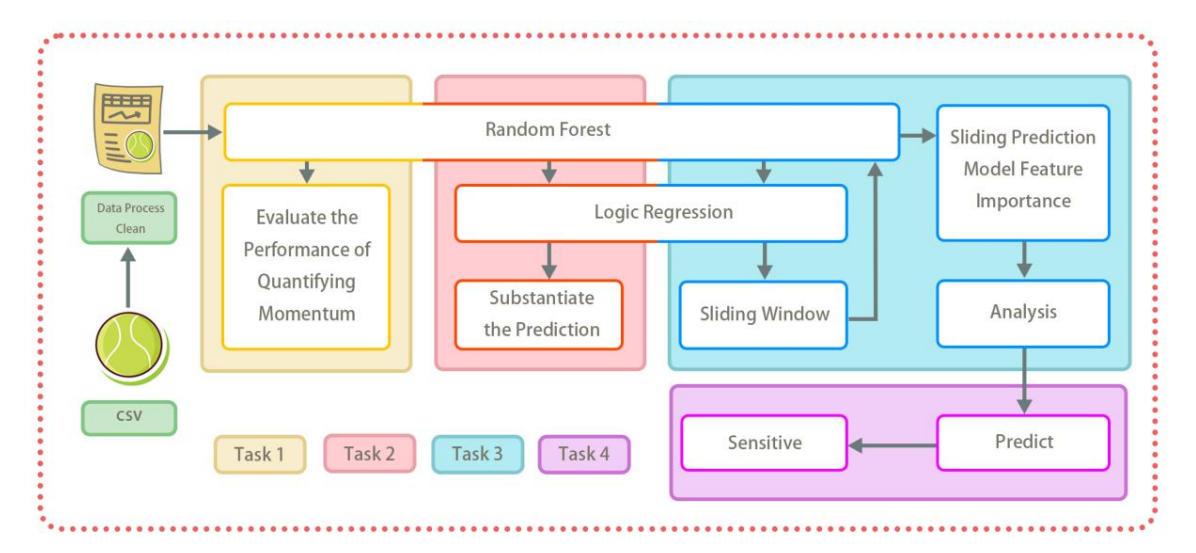
\includegraphics[width=12cm]{"C:/Users/admin/Desktop/GitHub/MCM/test/51XX/code/1.png"}
\caption{Work Process} \label{fig1}    
\end{figure}

\section{Assumptions and Justification}
\begin{itemize}
\item {\bf Athletes will not be affected by the results of previous matches while playing the
current match}. Supposing that the athlete is always in a good state of mind and that his or her
performance in the previous game does not affect the outcome of the current game.
        
\item {\bf Athletes have a fixed interval between each score}. Supposing the interval between goals
can be equated to the concept of time. In this way the time cost of scoring is quantifiable and
relatively stable in the tennis match and we can analyze game progression and athletes’ performance from a new perspective.

\end{itemize}

\section{Notations}

\setlength{\parindent}{2em} 
Table 1 shows the necessary notations and signs used in this paper. Other notations and signs
will be declared or defined when using.[2]

\newpage

\begin{table}[h] 
\centering  
\caption{Notations}  
\label{tab1} 
\begin{tabular}{ll} 
\toprule
Symbols  & Descriptions \\    
\midrule 
$S_{P1i}$ & player 1’s momentum integral value in one match\\
$S_{P2i}$ & player 2’s momentum integral value in one match\\
$A_r$   & service score rate                             \\
$F_r$   & service failure rate                           \\
$B_r$   & break success rate                             \\
$B_{fr}$  & break failure rate                             \\
\midrule 
$N_r$   & net scoring rate                               \\
\midrule 
$E_r$   & error ratio                                    \\
\midrule 
$T_s$   & the total number of serve in the set           \\
\midrule 
$M$     & momentum                                       \\

\bottomrule
\end{tabular}
\end{table}


\section{Data Preprocessing}
\subsection{Data Cleaning}

    The data cleaning processes are as follows.

    {\bf Overview of data sets: }This dataset is derived from the featured races of the Wimbledon
Championship and contains detailed race statistics. It is worth noting that there are a number of
missing values in the dataset, particularly in the $speed_mph$ (752 missing), $serve_width$ and
$serve_depth$ (54 missing each), and $return_depth$ (1309 missing) fields. \\

    {\bf Missing value handling:} In dealing with missing values in the dataset, special attention is
paid to the NA values in the speed column. In an initial check, 752 missing values were found in
the speed column. These missing values can occur for a variety of reasons, including data entry
errors or omissions during the data collection process. There were even instances in matches 1310
and 1311 where the whole bureau had unrecorded $rally_count$ as well as speed values.

    Further analysis showed that some of the missing speed values were associated with a
$rally_count$ of 0, which reflected a specific scenario of a no-ball exchange during the match, not
missing data, as shown in {\bf Figure 1}. In contrast, the missing data for complete matches may stem
from technical problems or human negligence in the recording process.

\begin{figure}[h]   
\centering          

\includegraphics[width=12cm]{"C:/Users/admin/Desktop/GitHub/MCM/test/51XX/code/2.png"}
\caption{$SpeedNA_Count_By_RallyCount$} \label{fig2}    
\end{figure} 
\newpage

    In the case of unrecorded data for an entire race, we decided to exclude these records from
the dataset given the non-direct impact of this data on model training. Data where a $rally_count$ of
0 resulted in a speed of 0 was considered a valid record and retained to accurately reflect the
reality of the race.

    Through this careful missing value handling strategy, we ensured the accuracy and reliability
of the data analysis and laid a solid foundation for the subsequent data analysis work. 

    {\bf Abnormal value progress:} In the dataset, there are 235 rows of records showing that when
double fault is 1, the serve\_width and serve\_depth fields are still recorded. Theoretically, in the
event of a double serve fault, the ball did not successfully cross the net and therefore the width and
depth of the serve should not be recorded.

\subsection{Data Cleaning}

    We find that serve\_no and speed are related. The box plot shows the distribution of serve
speeds according to the number of serves (first and second). The following points can be observed
from the graph:

\begin{figure}[h]   
\centering          
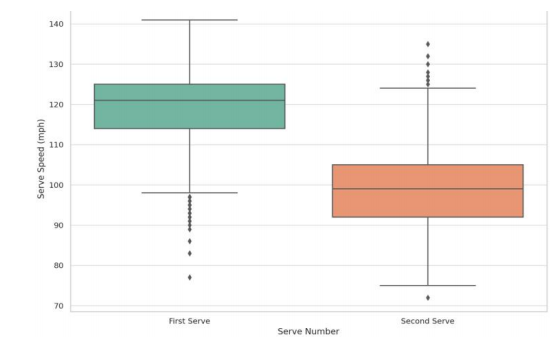
\includegraphics[width=12cm]{"C:/Users/admin/Desktop/GitHub/MCM/test/51XX/code/3.png"}
\caption{Boxplot of Serve Speed By Serve Number} \label{fig3}    
\end{figure} 
\newpage

    First serve speeds were typically higher than second serve speeds, reflecting a common
strategy in tennis whereby players tend to use more powerful serves on the first serve in an
attempt to score points outright or to gain a favorable position, while they tend to use more secure
serves on the second serve to avoid double faults. 

    The wider distribution of speeds on the first serve and the higher outliers at the top suggest
that players' serve speeds vary more when attempting more powerful serves. 

    The relatively more concentrated distribution of speeds and fewer outliers on the second
serve may be due to the fact that players focus more on accuracy and consistency on the second
serve to minimize the risk of double faults.

    These observations are consistent with the conventional strategy in tennis where the first
serve is more focused on aggressiveness while the second serve is more focused on insurance. This analysis helps us to gain a deeper understanding of players' serving strategies and their
potential impact on match outcomes.

\section{Model Construction}

\subsection{Discrete Performance Evaluating Model Based on Random Forest}

\subsubsection{Model Preparation}

    According to the requirements of problem 1, this paper needs to build a model to obtain the
scoring points occurring in the match. {\bf The Random Forest model} is chosen to determine the
weights of the indicators, therefore we are able to identify the better performance of the players
visually, then we apply the model to as many games as possible.

\begin{itemize}
\item {\bf Firstly, we acquire data information such as “ace” or “net\_pt”} , which refer to a not- served shot and a player’s position separately from the provided data set, result data of each set
or game can also be found.
        
\item {\bf Next, we try to design a model to quantify “momentum”}. Momentum can be perceived as
strength or force during a match, since it is difficult to quantize, so we attempt to incorporate the
Calculation of short-term indicators, transforming scoring concepts into momentum indicators.
    
\item {\bf Then, we discover that momentum is usually reflected as a change in game
performance over a short period of time}. For example, consecutive scores can be seen as a
direct reflection of momentum. By calculating short-term changes in scoring for each point
(e.g., consecutive points, short-term serve success and break rates, etc.), these short-term
performances can be quantified as indicators of momentum.

\end{itemize}

\subsubsection{Random Forest Model}

    Although the ultimate goal is to predict the outcome of the game, the impact of momentum
changes on the outcome of the game can be revealed by analyzing the relationship between short-term momentum indicators and the final outcome of the game. Short-term momentum indicators
can be trained as features and match results (win/lose) as labels in the model to determine the
association between momentum and match. 

    We can begin to quantify indicators by virtue of the above idea, but it is not yet possible to
determine the specific levels of quantification. We then use a random forest model to analyze the
importance of the characteristics of these indicators. 

    Random Forest is a supervised algorithm that uses an integrated learning method consisting
of numerous decision trees. It’s able to handle large and complex datasets, including multiple
types of variables, which is useful for analyzing the impact of various factors in tennis matches. What is more, it can provide an effective method for assessing the importance of individual
features in predicting outcomes, which allows to identify which factors have the greatest impact
on player momentum and match results.[4]

\begin{figure}[h]   
\centering          
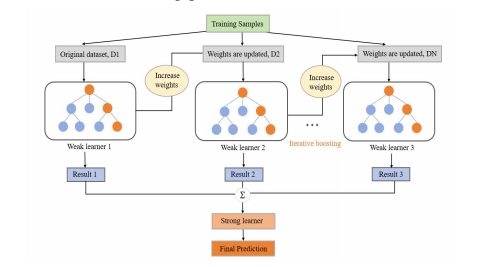
\includegraphics[width=12cm]{"C:/Users/admin/Desktop/GitHub/MCM/test/51XX/code/4.png"}
\caption{Concept of Random Forest} \label{fig4}    
\end{figure} 

    Therefore we try to describe the method by means of detail principles of the Random Forest
model, including how it handles large numbers of input variables and evaluates the importance of
features. We can explain the source of the dataset, the variables chosen (e.g., score, serve success
rate, unforced errors, etc.), and how the data were prepared for use in the analysis accordingly. 

    We focus on the characteristic importance scores of each factor's impact on the outcome of
the match. Specially, we weight the “serve” artificially low. 

    The results of the Random Forest Model analysis are in the following graphs

\begin{table}[h] 
\centering  
\caption{Feature Importance Ranking in Random Forest Model} 
\label{tab2} 
\begin{tabular}{ccc} 
\toprule  
Order      & Features   & Weights  \\
\midrule  
1  & break\_pt & 0.275942 \\ 
2  & point\_victor & 0.168837 \\
3  & unf\_err & 0.139420 \\
4  & winner & 0.108685 \\
5  & ace & 0.095252 \\
6  & double\_fault & 0.077130 \\
7  & net\_pt & 0.074068 \\
8  & net\_pt\_won & 0.039238 \\
9  & break\_pt\_missed & 0.021428 \\

\bottomrule  %画底部横线
\end{tabular}
\end{table}

\begin{figure}[h]   
\centering          
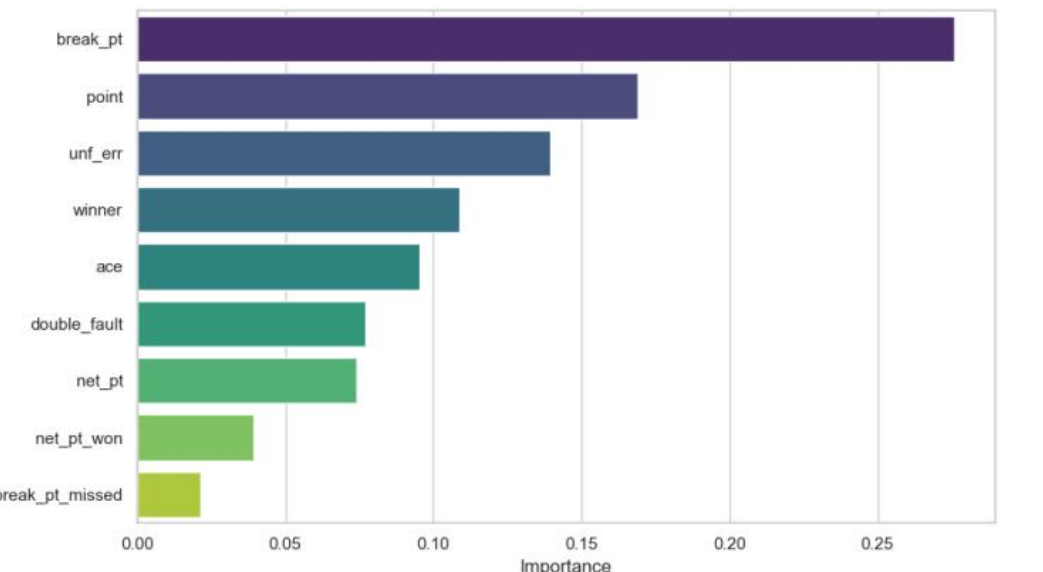
\includegraphics[width=12cm]{C:/Users/admin/Desktop/GitHub/MCM/test/51XX/code/10.png}
\caption{Feature Importance in Random Forest Model} \label{fig5}    
\end{figure}

\begin{equation} \label{eq1}
\text{According to the chart presented above, we define the following weights: } \\
W = (0.275942, 0.8 \times 0.168837, -0.139420, 0.108685, -0.095252, 0.077130, 0.074068, 0.074068, -0.021428)
\end{equation}

\begin{equation} \label{eq2}
M = \sum_{i=1}^{9} (W_i \times \alpha_i)
\end{equation}


\begin{figure}[h]
    \centering
    \begin{subfigure}{0.45\textwidth}  
        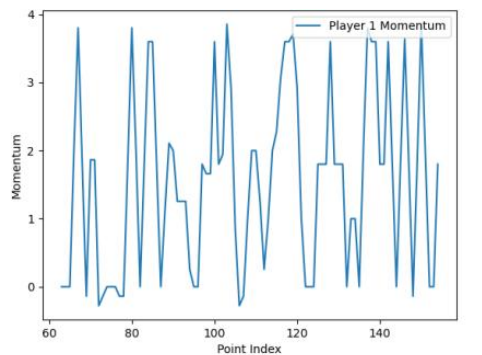
\includegraphics[width=\textwidth]{C:/Users/admin/Desktop/GitHub/MCM/test/51XX/code/6.png}
        \caption{First Image}  
        \label{fig:first}
    \end{subfigure}
    \hfill
    % 插入第二张图片
    \begin{subfigure}{0.45\textwidth}
        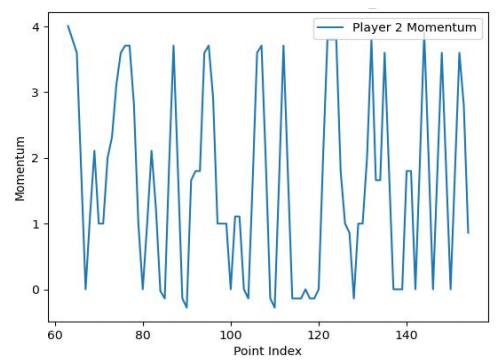
\includegraphics[width=\textwidth]{C:/Users/admin/Desktop/GitHub/MCM/test/51XX/code/6.2.png}
        \caption{Second Image}  % 为第二张图片添加标题
        \label{fig:second}
    \end{subfigure}
    
    \caption{Player 1/2’s Momentum in this set\_no} 
    \label{fig:twoimages}
\end{figure}

    These two images above show the performance for the players themselves:

\begin{figure}[h]   
\centering          
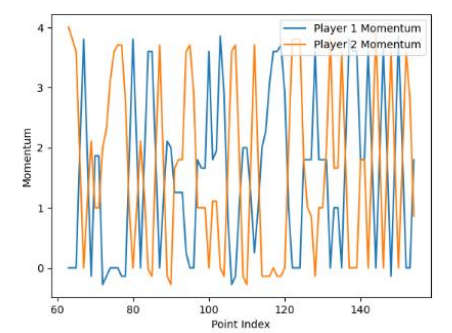
\includegraphics[width=0.5\textwidth]{C:/Users/admin/Desktop/GitHub/MCM/test/51XX/code/7.png}
\caption{Player 1’s vs Player 2’s Momentum Comparison in the set\_no} \label{fig6}    
\end{figure} 

    This picture above reflects the fact that the momentum values of the two players are in a state
of waxing and waning, which basically corresponds with players’ actual state in a real game.[3]
\newpage

\begin{figure}[h]   
\centering          
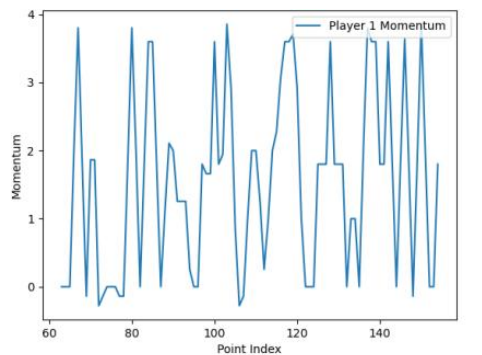
\includegraphics[width=0.5\textwidth]{C:/Users/admin/Desktop/GitHub/MCM/test/51XX/code/6.png}
\caption{: Player 1-Player’s Momentum Difference Comparison in this set\_no} \label{fig7}    
\end{figure} 

    This picture above shows that in which time period which athlete performs better. For
example, the red spot in the diagram indicates that at the 78-minute mark of the opening, Player
1’s momentum minus player 2’s momentum is negative, which represents clearly that at this time, player 2 performs better than player 1.

\begin{figure}[h]
    \centering
    \begin{subfigure}{0.45\textwidth}  
        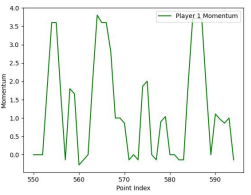
\includegraphics[width=5cm, height=4cm]{C:/Users/admin/Desktop/GitHub/MCM/test/51XX/code/11.1.png}  
        \label{fig:first}
    \end{subfigure}
    \hfill
    \begin{subfigure}{0.45\textwidth}
        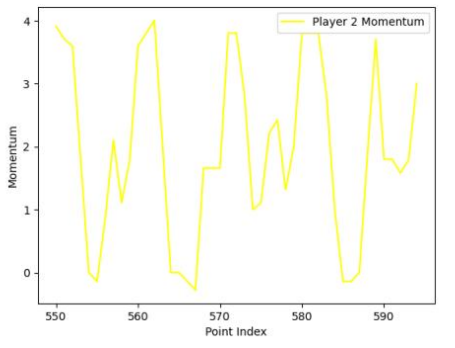
\includegraphics[width=5cm, height=4cm]{C:/Users/admin/Desktop/GitHub/MCM/test/51XX/code/11.2.png}
        \label{fig:second}
    \end{subfigure}\\
    \begin{subfigure}{0.45\textwidth}  
        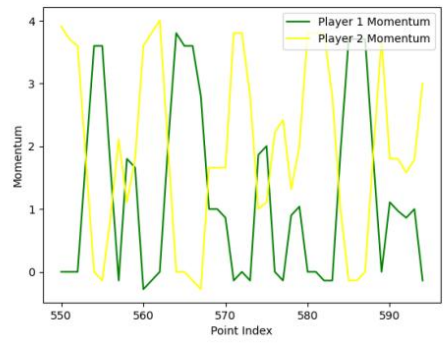
\includegraphics[width=5cm, height=4cm]{C:/Users/admin/Desktop/GitHub/MCM/test/51XX/code/11.3.png}  
        \label{fig:third}
    \end{subfigure}
    \begin{subfigure}{0.45\textwidth}  
        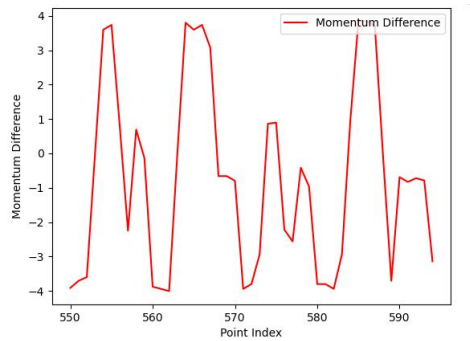
\includegraphics[width=5cm, height=4cm]{C:/Users/admin/Desktop/GitHub/MCM/test/51XX/code/11.4.png}  
        \label{fig:forth}
    \end{subfigure}
    
    \caption{Player 1/2’s Momentum in this set\_no} 
    \label{fig:twoimages}
\end{figure}

\subsection{Assessment Based on Logistic Regression}

\subsubsection{Assessment Preparation}

    According to the requirements of the problem, this paper needs to assess that “momentum”
actually plays an role in a match and swings in play and runs of success by one player are not
random but correlative. We choose {\bf Logistic Regression in classification algorithms} to train the
model, then we can obtain the training results with higher predicted value. Finally we are able to
visualize the description based on the model results to prove the crucial role “momentum” acts in
the match and its high relevancy.  

    Through the weight we determine in the previous question, we are able to derive two chart
with its horizontal axis coordinates are the number of points scored per game and the vertical axis
coordinates are the momentum values for each player. Then we integrate the momentum value
folds in the two charts separately

\begin{figure}[h]   
\centering          
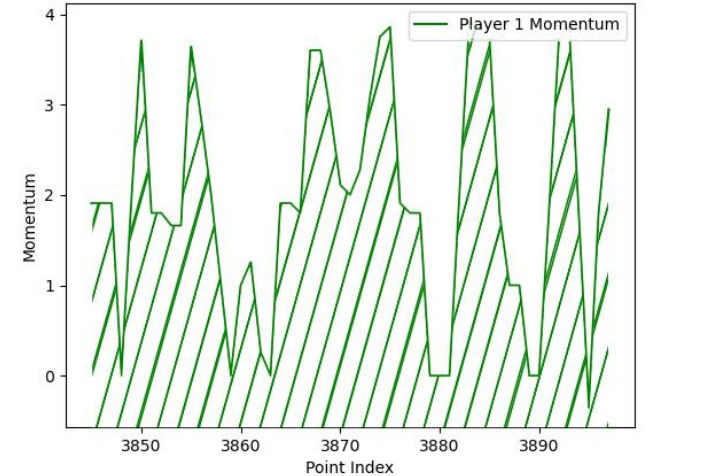
\includegraphics[width=0.5\textwidth]{C:/Users/admin/Desktop/GitHub/MCM/test/51XX/code/12.png}
\caption{Player 1’s Momentum in this set\_no} \label{fig7}    
\end{figure} 

    Accordingly, we can acquire the total momentum value for each player. 
    By analogy with the definition “work” in physics, we figure that momentum can also
accumulate over time, so we define three values: $S_{p1}$,$S_{p2}$,$X{i}$
    In the same way, we accordingly integral to get the cumulative value of the momentum of the
two athletes in the current match, so we build this model:  

\begin{equation} \label{eq3}
    X{i} = \frac{S_{p1}}{S_{p2}+S_{p1}}
\end{equation}

    Since there are many rounds in the competition, the momentum performance of the athletes
will vary accordingly, so there will be multiple $X_i$,$Y_i$ represents the results of the set, we stipulate
that :

\begin{equation} \label{eq4}
    Y{i} = 0, P_1  lost the set
\end{equation}

\begin{equation} \label{eq5}
    Y{i} = 1, P_1   won the set
\end{equation}

    So we can capture series of dataset ($X_i$,$Y_i$)

    Through the original data scatter plot, we notice that the distribution of $X_i$ is quite compact, so we choose to standardize $X_i$ to make it more discrete, as it shown in the following diagram:

\begin{figure}[h]
    \centering
    \begin{subfigure}{0.45\textwidth}  
        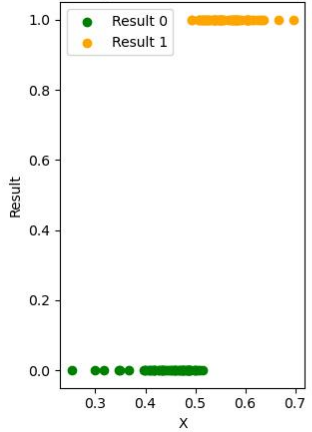
\includegraphics[width=7cm, height=10cm]{C:/Users/admin/Desktop/GitHub/MCM/test/51XX/code/13.1.png}
        \caption{Original Data Scatter Plot}  
        \label{fig:first}
    \end{subfigure}
    \hfill
    \begin{subfigure}{0.45\textwidth}
        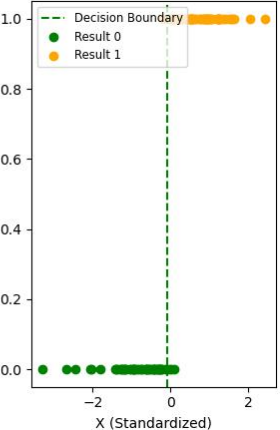
\includegraphics[width=7cm, height=10cm]{C:/Users/admin/Desktop/GitHub/MCM/test/51XX/code/13.3.png}
        \caption{Standardized Data Scatter Plot} 
        \label{fig:second}
    \end{subfigure}
        
    \caption{Two Types of Data Scatter} 
    \label{fig:twoimages}
\end{figure}

    We then use {\bf Logistic Regression:}

\begin{equation} \label{eq6}
\vec{W}\leftarrow \vec{W}+\eta\sum_{i=1}^{n}\frac{y_i\vec{x_i}}{1+exp(y_i\vec{w}\cdot\vec{x_i})}
\end{equation}


\end{document}

%\begin{figure}[h]   
%\centering          
%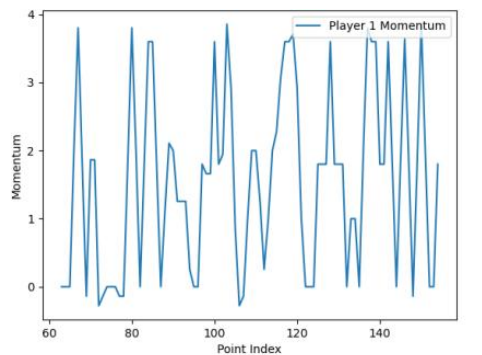
\includegraphics[width=\textwidth]{C:/Users/admin/Desktop/GitHub/MCM/test/51XX/code/6.png}
%\caption{Boxplot of Serve Speed By Serve Number} \label{fig6}    
%\end{figure} 

%\begin{figure}[h]   
%\centering          
%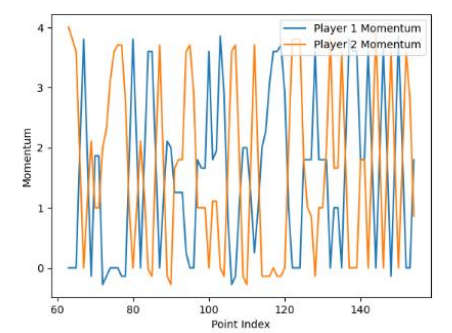
\includegraphics[width=12cm]{C:/Users/admin/Desktop/GitHub/MCM/test/51XX/code/7.png}
%\caption{Player 1's vs Player 2's Momentum Comparison in the $set_no$} \label{fig7}    
%\end{figure}

%This picture above reflects the fact that the momentum values of the two players are in a state
%of waxing and waning, which basically corresponds with players’ actual state in a real game.[3]

%\begin{figure}[h]   
%\centering          
%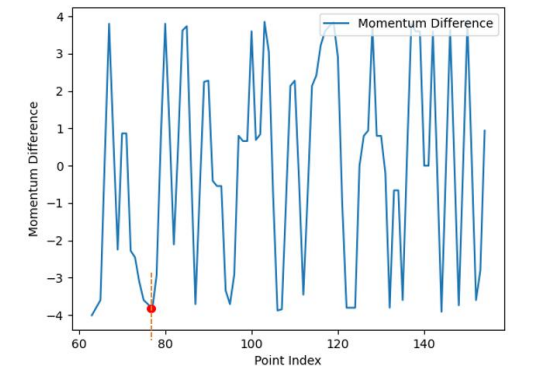
\includegraphics[width=12cm]{"C:/Users/admin/Desktop/GitHub/MCM/test/51XX/code/8.png"}
%\caption{Player 1-Player’s Momentum Difference Comparison in this $set_no$} \label{fig7}    
%\end{figure}
%This picture above shows that in which time period which athlete performs better. For
%example, the red spot in the diagram indicates that at the 78-minute mark of the opening, Player
%1’s momentum minus player 2’s momentum is negative, which represents clearly that at this time, player 2 performs better than player 1.

%picture insert

%\subsection{Assessment Based on Logistic Regression}
%\subsubsection{Assessment Preparation}

%    According to the requirements of the problem, this paper needs to assess that “momentum”
%actually plays an role in a match and swings in play and runs of success by one player are not
%random but correlative. We choose Logistic Regression in classification algorithms to train the
%model, then we can obtain the training results with higher predicted value. Finally we are able to
%visualize the description based on the model results to prove the crucial role “momentum” acts in
%the match and its high relevancy
%    Through the weight we determine in the previous question, we are able to derive two chart
%with its horizontal axis coordinates are the number of points scored per game and the vertical axis
%coordinates are the momentum values for each player. Then we integrate the momentum value
%folds in the two charts separately. 

%\begin{figure}[h]   
%\centering          
%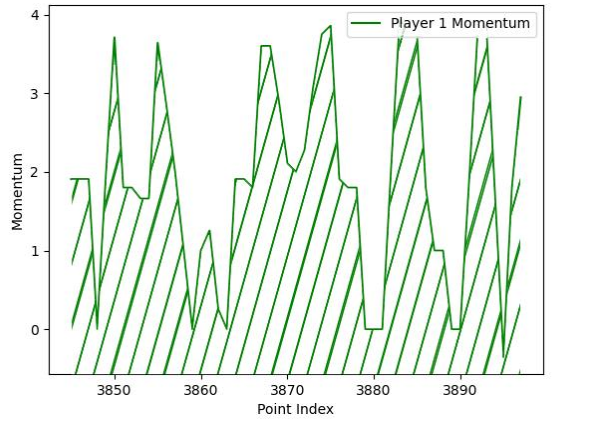
\includegraphics[width=12cm]{C:/Users/admin/Desktop/GitHub/MCM/test/51XX/code/9.png}
%\caption{Player 1’s Momentum in this $set_no$} \label{fig9}    
%\end{figure}

%    Accordingly, we can acquire the total momentum value for each player. 
%    By analogy with the definition “work” in physics, we figure that momentum can also
%accumulate over time, so we define three values: $S_{p1}$,$S_{p2}$,$X_i$
%    In the same way, we accordingly integral to get the cumulative value of the momentum of the
%two athletes in the current match, so we build this model:
   
%\begin{equation} \label{eq1}
%\text{According to the chart presented above, we define the following weights: } \\
%W = (0.275942, 0.8 \times 0.168837, -0.139420, 0.108685, -0.095252, 0.077130, 0.074068, 0.074068, -0.021428)
%\end{equation}
%Since there are many rounds in the competition, the momentum performance of the athletes
%will vary accordingly, so there will be multiple ��, �� represents the results of the set, we stipulate
%that :

%X_i = S_{p1i}/(S_{p1i}+S_{p2i})

